\chapter{Экспериментальная часть часть}

\section{Демонстрация работы программы}
На рисунке 4 представлена работы программы. В консоль выводится результат подсчёта расстояний для каждого из алгоритмов, а для алгоритмов, использующих матрицу - также выводится и матрица.

\begin{figure}[hp]
    \begin{center}
        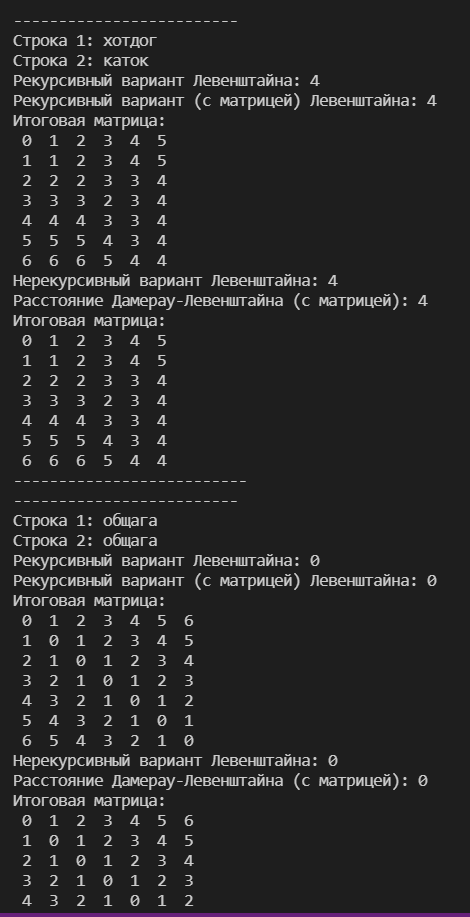
\includegraphics[scale = 0.8]{inc/demonstrate.PNG}
    \end{center}
    \caption{Демонстрация работы алгоритма}
\end{figure}
\clearpage

\section{Технические характеристики}
Технические характеристики устройства, на котором производилось тестирование:
\begin{itemize}
    \item операционная система: Windows 10;
    \item оперативная память: 8 ГБ;
    \item процессор: Intel Core i5-1135G7 @ 2.40GHz.
\end{itemize}

Тестирование производилось на ноутбуке при включённом режиме производительности. Во время тестирования ноутбук был загружен только системными процессами.

\section{Время работы алгоритмов}
Алгоритмы тестировались с помощью функции process\_time\_ns из библиотеки time. Чтобы время удалось отследить и результаты были достаточно точными, каждый тест проводится N=100 раз, после чего общее время делится на 100 - тогда получится среднее время работы каждого алгоритма по одному тесту. Для каждого теста генерировалась случайным образом строка из M символов.

Результаты представлены в таблице 4.1. Пропущенное значение означает, что для таких параметров тестирование не проводилось.

\begin{table}[!ht]
  \caption{Сравнительная таблица времени работы алгоритмов (время в нс)}
  \centering
\begin{tabular}{ | l | l | l | l | l |}
\hline
Размер & Итер. & Рекурс.(с матрицей)  & Рекурс. & Дамерау \\ \hline
0 & 3125 & 4687 & 1562 & 4687\\
1 & 6250 & 12500 & 6250 & 14062 \\
2 & 10937 & 29687 & 28125 & 39062 \\
3 & 15625 & 59375 & 125000 & 75000\\ 
4 & 23437 & 93312 & 620312 & 99375 \\
5 & 28456 & 95750 & 2312500 & 103750 \\
6 & 32812 & 167187 & 17723437 & 237500\\ 
7 & 56250 & 259375 & 93750000 & 421875\\
8 & 78125 & 421875 & 734375000 & 484375\\
9 & 95000 & 473500 & 12062500000 & 540605\\
10 & 109375 & 515625 & 14890625000 & 625000\\
15 & 312500 & 1562500 & - & 2187500 \\
20 & 468750 & 2656250 & - & 3281250 \\
25 & 647850 & 3593750 & - & 4843750\\
30 & 937500 & 5625000 & - & 7500000\\
35 & 1250000 & 6562500 & - & 9531250 \\
40 & 1875000 & 8593750 & - & 12500000 \\
45 & 2362500 & 10312500 & - & 15312500 \\
50 & 2875000 & 12968750 & - & 24062500 \\
60 & 3906250 & 21718750 & - & 31093750 \\
70 & 4687500 & 28437500 & - & 42812500 \\
80 & 7531250 & 53437500 & - & 55625000 \\
90 & 10312500 & 69375000 & - & 69218750 \\
100 & 14625000 & 77500000 & - & 92656250 \\
\hline
\end{tabular}
\end{table}



\clearpage


\begin{figure}[hp]
    \centering
    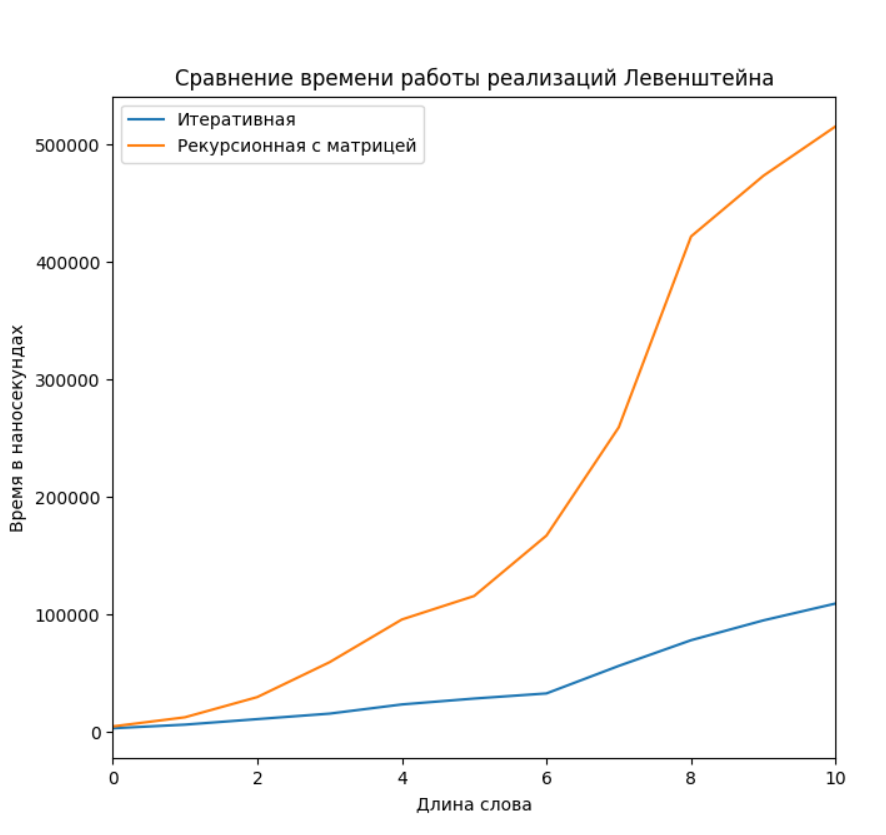
\includegraphics[width=\linewidth]{inc/compare1.png}
    \caption{Сравнительный график времени работы итерационного и рекурсивного алгоритмов нахождения расстояния Левенштейна}
\end{figure}
\clearpage

\begin{figure}[hp]
    \centering
    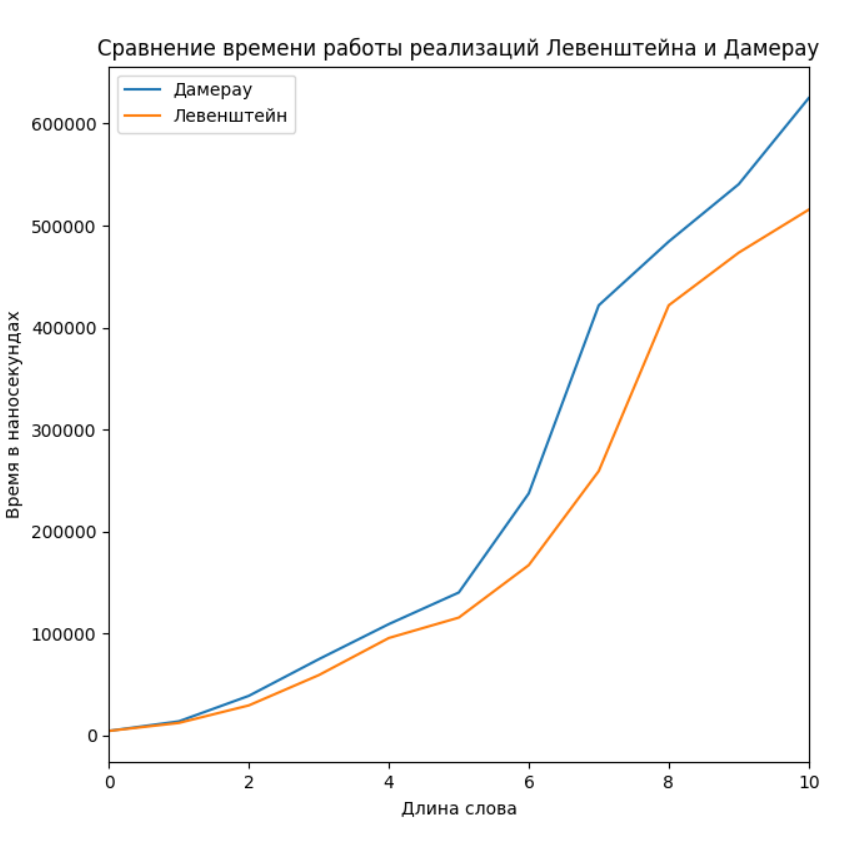
\includegraphics[width=\linewidth]{inc/compare2.png}
    \caption{Сравнительный график времени работы одинаковых алгоритмов поиска расстояния Левенштейна и расстояния Дамерау-Левенштейна}
\end{figure}
\clearpage
\section{Использование памяти}

Алгоритмы Левенштейна и Дамерау — Левенштейна не отличаются друг от друга с точки зрения использования памяти, следовательно, достаточно рассмотреть лишь разницу рекурсивной и матричной реализаций этих алгоритмов.

Максимальная глубина стека вызовов при рекурсивной реализации равна сумме длин входящих строк, соответственно, максимальный расход памяти (\ref{for:99})
\begin{equation}
(\mathcal{C}(S_1) + \mathcal{C}(S_2)) \cdot (2 \cdot \mathcal{C}\mathrm{(string)} + 3 \cdot \mathcal{C}\mathrm{(int)}),
\label{for:99}
\end{equation}
где $\mathcal{C}$ — оператор вычисления размера, $S_1$, $S_2$ — строки, $\mathrm{int}$ — целочисленный тип, $\mathrm{string}$ — строковый тип.

Использование памяти при итеративной реализации теоретически равно
\begin{equation}
(\mathcal{C}(S_1) + 1) \cdot (\mathcal{C}(S_2) + 1) \cdot \mathcal{C}\mathrm{(int)} + 7\cdot \mathcal{C}\mathrm{(int)} + 2 \cdot \mathcal{C}\mathrm{(string)}.
\end{equation}

Но в случае хранения двух строк количество потребляемой памяти резко падает:
\begin{equation}
(\mathcal{C}(S_2) + 1) \cdot 3 \cdot \mathcal{C}\mathrm{(int)} + 7\cdot \mathcal{C}\mathrm{(int)} + 2 \cdot \mathcal{C}\mathrm{(string)}.
\end{equation}


\section{Вывод}

Рекурсивный алгоритм Левенштейна работает на порядок дольше итеративных реализаций, время его работы увеличивается в геометрической прогрессии. 
На словах длиной 10 символов, матричная реализация алгоритма Левенштейна превосходит по времени работы рекурсивную в 160000 раз. 
Рекурсивный алгоритм с заполнением матрицы превосходит простой рекурсивный на аналогичных данных в 29000 раз. 
Алгоритм Дамерау — Левенштейна по времени выполнения выполняется медленнее, чем аналогичная реализация алгоритма Левенштейна. 
В нём добавлены дополнительные проверки, и по сути он является алгоритмом другого смыслового уровня.

По расходу памяти классический итерационный алгоритм проигрывает рекурсионному, но в случае оптимизации итерационный алгоритм становится выигрышней по памяти, чем рекурсионные аналоги.